\documentclass[a4paper,11pt]{report}
\usepackage[left=3cm, right=3cm, top=3cm, bottom=3cm]{geometry}
\usepackage{graphicx}
\usepackage{listings}
\usepackage{titlesec}
\usepackage{fancyhdr}
\usepackage{epstopdf}
\usepackage{float}
\usepackage{amsmath}
\usepackage{setspace}
\usepackage{eufrak}
\usepackage{url}
\usepackage{listings}
\usepackage{courier}
\usepackage{hyperref}
 \newcommand{\textform}[1]{\fontsize{14}{20}\selectfont{#1}}
\pagestyle{fancy}
\fancyhf{}
\fancyhead[R]{\thepage}
\renewcommand{\chaptermark}[1]{\markboth{#1}{}}
\renewcommand{\headrulewidth}{1pt}
\renewcommand{\footrulewidth}{1pt}

\lhead{\footnotesize{ACCREDIFY}}
\rhead{}
\lfoot{\footnotesize{Department of Computer Science \& Engg.}}
\cfoot{}
\rfoot{\thepage}

\titleformat{\chapter}[display]
{\normalfont\Large\bfseries\centering}{\chaptertitlename\
\thechapter}{20pt}{\Large}

\begin{document}

\thispagestyle{empty}
  \begin{center}
      \fontsize{22}{25}\selectfont{\textbf{GOVERNMENT POLYTECHNIC COLLEGE PERUMBAVOOR}}\\[.1cm]
            \fontsize{15}{25}\selectfont{\textbf{Koovappady P.O Ernakulam-683 544 Kerala
    }}\\[1.2cm]
\begin{figure}[h]
	\centering
	\hspace{21pt}
	
\includegraphics[width=.50\linewidth]{logo.png}
	\label{fig:logo.png}
\end{figure}

\fontsize{14}{25}\selectfont{\textbf{Semester - VI}}\\
\fontsize{14}{25}\selectfont{\textbf{Computer Engineering 2022-23}}\\[1.2cm]

\fontsize{14}{25}\selectfont{\textbf{PROJECT REPORT}}\\[.1cm]
    \fontsize{14}{25}\selectfont{on}\\
    \fontsize{20}{25}\selectfont{\textbf{ACCREDIFY}}\\[.1cm]
    \fontsize{14}{25}\selectfont{\textbf{AN ACCREDITATION MANAGEMENT SYSTEM}}\\[1.2cm]
    \fontsize{12}{25}\selectfont{\textbf{Submitted by}}\\[.2cm]
    \fontsize{14}{25}\selectfont \bfseries{VISHNU SURESH}\\[.1cm]
    \fontsize{12}{25}\selectfont{\textbf{20130132}}\\[.2cm]
%\vfill
 \end{center}

\fontsize{12pt}{20}\selectfont
\thispagestyle{empty}


\newpage
  \thispagestyle{empty}

    \begin{center}
      \fontsize{14}{20}\selectfont \textbf{GOVERNMENT POLYTECHNIC COLLEGE PERUMBAVOOR}\\
     
    \fontsize{14}{20}\selectfont \textbf{
DEPARTMENT OF COMPUTER ENGINEERING}\\[1.5cm]
\begin{figure}[h]
\centering
	\hspace{.5cm}

\includegraphics[width=0.3\linewidth]{logo.png}
	\label{fig:logo.png}
\end{figure}

     
      \textbf{CERTIFICATE}
    \end{center}
    \vspace{.5cm}
    \textform{This is to certify that the project report entitled \textbf{Accredify - The Accreditation Management System} submitted by \textbf{Vishnu Suresh} is approved for submission requirement for 6009 -Project and Seminar in  $6^{th}$ semester Computer Engineering at Govt.Polytechnic College,Perumbavoor.}\\[0.15cm]


\begin{minipage}{.40\textwidth}
    \begin{flushleft}
        \begin{center}
            \fontsize{12}{25}\selectfont{\textbf{Head of Section}}\\[1.5cm] 
        \end{center}
    \end{flushleft}
\end{minipage}
\hfill
\begin{minipage}{0.40\textwidth}
    \begin{flushright}
        \begin{center}
            \fontsize{12}{25}\selectfont{\textbf{Lecturer in Charge}}\\[1.5cm]
        \end{center}
    \end{flushright}
\end{minipage}




\vspace{1cm}
\begin{flushleft}
  \fontsize{12}{20}\selectfont \textbf{Date  :}\\
  \fontsize{12}{20}\selectfont \textbf{Place :}
\end{flushleft}
\vspace{1cm}
\begin{minipage}{.4\textwidth}
    \begin{flushleft}
    \begin{center}
    
    \fontsize{14}{25}\selectfont \bfseries{Internal Examiner}\\[.1cm]
    
%\vfill
 \end{center}
    \end{flushleft}
      \end{minipage}
\begin{minipage}{0.8\textwidth}
\begin{flushright}
\begin{center}
 
%\vfill
\fontsize{14}{25}\selectfont \bfseries{External Examiner}\\[.1cm]

\end{center}
\end{flushright}
\end{minipage}

\newpage
\fontsize{12pt}{20}\selectfont
\thispagestyle{empty}
  \renewcommand\abstractname{\textform{\textbf{ACKNOWLEDGMENT}}}
    \begin{abstract}
      \vspace{2.5cm}
      
         I would like to express my sincere gratitude to all those who have contributed to the successful completion of my project Accredify - The Accreditation Management Application. This opportunity has allowed me to delve into a fascinating field of web development and expand my knowledge in computer engineering.

First and foremost, I extend my heartfelt appreciation to Dr. Aiju Thomas, the Principal of Government Polytechnic College Perumbavoor. I am grateful for his constant support, guidance, and encouragement throughout my academic journey. His visionary leadership and commitment to excellence have created an environment conducive to learning and exploration.

I am indebted to Mr. Biju Peter, the Head of the Department of Computer Engineering, for his invaluable guidance and mentorship. His expertise, patience, and enthusiasm have been instrumental in shaping my understanding of the subject and honing my research skills. I am thankful for his unwavering support and valuable insights.

I would also like to acknowledge the faculty members of the Computer Engineering Department for their constant support and encouragement throughout my academic journey. Their expertise and passion for teaching have played a significant role in shaping my intellectual growth.

I would like to express my gratitude to my classmates and team members for their support and encouragement. Their presence and collaboration have made the learning experience enjoyable and memorable.

Thank you all for your unwavering support and belief in me.
    \end{abstract}
 

  \tableofcontents
\thispagestyle{empty}

\chapter{Introduction}

\paragraph{}Accreditation plays a crucial role in assessing and ensuring the quality and standards of educational institutions. However, the accreditation process can be complex and time-consuming, requiring meticulous evaluation and compliance with various standards and criteria.

To address these challenges, Accredify web application provides a  platform where college departments can easily navigate the accreditation process. Departments can create individual accounts and access a range of features and resources designed to support their accreditation journey. The system offers a structured assessment framework that enables departments to evaluate their readiness for accreditation. By providing a comprehensive set of criteria and guidelines, the system assists departments in identifying areas of improvement and implementing necessary measures to meet accreditation standards.

A key aspect of the system is the integration of pricing and consultation services. Departments that opt for a paid subscription gain access to advanced consultation services, where experienced professionals provide personalized guidance and support. This additional layer of expertise ensures that departments receive tailored assistance in addressing specific challenges and enhancing their accreditation preparedness.

Furthermore, the system incorporates an admin portal that empowers administrators to gain valuable insights into departmental data. Administrators can visualize key metrics such as admissions and graduations per year, enabling them to monitor performance trends and make informed decisions to further improve the quality of education within the institution.

Overall, the Accreditation Management System aims to simplify and streamline the accreditation process for college departments. It promotes collaboration, provides valuable resources, and offers expert guidance to ensure that departments are well-equipped to meet accreditation standards. By leveraging the power of the MERN stack, the system delivers a user-friendly and efficient solution that contributes to the pursuit of academic excellence within educational institutions.
  

  
\chapter{Problem Statement}
The Accreditation Management System aims to address several challenges and problems commonly faced by college departments during the accreditation process. Some of the key problems that this application seeks to solve include:	

\section{Manual and Time-Consuming Process}
Traditional accreditation processes often involve extensive paperwork, manual data entry, and complex administrative tasks. This application automates and streamlines these processes, reducing the time and effort required for accreditation.
\section{Lack of Clarity and Guidance}
Many college departments struggle with understanding the accreditation standards and requirements. The application provides a clear framework and guidelines, helping departments assess their readiness and take necessary steps for compliance.
\section{Limited Self-Assessment Capabilities}
Without proper tools and resources, departments may struggle to conduct a comprehensive self-assessment of their strengths and weaknesses. The application offers self-assessment features, enabling departments to identify areas of improvement and develop actionable plans.
\section{Insufficient Data Analysis}
Analyzing departmental data, such as admissions and graduations, is crucial for identifying trends and making informed decisions. The application's data visualization and analysis capabilities help administrators gain valuable insights into departmental performance and identify areas for enhancement.
\section{Communication and Collaboration Challenges}
Coordinating accreditation-related tasks and fostering collaboration among department members can be challenging. The application provides a centralized platform for communication, document sharing, and task management, promoting efficient collaboration and seamless information exchange.
\section{Lack of Advanced Consultation}
Departments may require expert guidance and consultation to navigate complex accreditation requirements. The application offers advanced consultation services, providing specialized support and personalized advice to assist departments in meeting accreditation standards.

\chapter{Solutions}
The Accredify offers a range of solutions to address the challenges faced by college departments during the accreditation process. Some of the key solutions provided by this application include:
\section{Streamlined Accreditation Process}
The application simplifies and automates various accreditation-related tasks, such as document submission, data collection, and assessment. This streamlines the overall process, reducing manual effort and improving efficiency.
\section{Comprehensive Guidelines and Standards}
The application provides departments with clear and up-to-date accreditation guidelines and standards. It helps departments understand the requirements, criteria, and benchmarks they need to meet for successful accreditation.
\section{Self-Assessment Tools}
The application offers self-assessment features that enable departments to evaluate their performance against accreditation standards. It provides assessment questionnaires, checklists, and performance indicators to help departments identify their strengths and areas for improvement.
\section{Data Visualization and Analysis}
The application includes data visualization and analysis tools that allow administrators to view and analyze departmental data, such as admissions, graduations, and performance metrics. This helps in identifying trends, patterns, and areas that require attention.
\section{Collaboration and Communication Platform}
The application serves as a centralized platform for departments to collaborate, communicate, and share documents related to accreditation. It facilitates seamless communication among department members, streamlines document management, and ensures easy access to relevant information.
\section{Advanced Consultation Services}
Departments that opt for the paid services receive advanced consultation from accreditation experts. This includes personalized guidance, advisory support, and assistance in meeting accreditation requirements effectively.

\chapter{Requirement Analysis}
\section{Computer Specifications}
\begin{itemize}
  \item A computer with a minimum of 8 GB RAM is recommended to ensure smooth performance during development and execution of the project.
  \item Adequate processing power and storage capacity are required to handle the project files and related dependencies.
\end{itemize}

\section{Operating System}
\begin{itemize}
  \item The project can be developed and executed on various operating systems, including Windows, macOS, or Linux, as long as the necessary software dependencies are supported.
\end{itemize}

\section{Node.js}
\begin{itemize}
  \item Node.js runtime environment is a prerequisite for running the project. It should be installed on the computer.
  \item The recommended version of Node.js may vary depending on the specific project requirements and dependencies. Please refer to the project documentation or requirements for the appropriate Node.js version.
\end{itemize}

\section{Dependencies and Libraries}
\begin{itemize}
  \item The project may rely on specific libraries, frameworks, or packages. These dependencies should be installed according to the project's requirements.
  \item It is essential to ensure that the required versions of these dependencies are compatible with the project's codebase and specifications.
\end{itemize}

\section{Development Tools}
\begin{itemize}
  \item An integrated development environment (IDE) or a text editor of your choice should be available to facilitate code editing and development.
  \item Git, a version control system, is recommended for managing source code revisions, collaborating with team members, and tracking project changes.
\end{itemize}

\section{Internet Connectivity}
\begin{itemize}
  \item Although not mandatory for the core functionality of the project, internet connectivity may be required for installing dependencies, accessing external APIs, or utilizing cloud-based services.
\end{itemize}
It is crucial to review and fulfill these system requirements to ensure a smooth setup and execution of the project. Additionally, regularly updating the dependencies and software versions as recommended by the project maintainers will help maintain compatibility and security.


\chapter{Technologies used}

Accredify utilizes the MERN stack for full stack web development and razorpay for payment integration.

\section{MongoDB}
MongoDB is an open-source, NoSQL database management system that is designed to handle large volumes of unstructured and semi-structured data. It utilizes a flexible document-oriented approach, storing data in JSON-like documents called BSON. This allows for easy manipulation and querying of data, providing schema flexibility and accommodating evolving data requirements. MongoDB excels in scalability, allowing for horizontal scaling by distributing data across multiple servers or shards. It also offers high performance with optimization techniques such as indexing, sharding, and in-memory caching. MongoDB supports a powerful query language with advanced filtering, sorting, and aggregation capabilities, enabling efficient data retrieval and analysis. Application uses mongodb cloud for data storage.

\section{Express.js}
Express.js is a minimalistic and flexible web application framework for Node.js. It provides a robust set of features and functionalities that simplify the development of web applications and APIs. With its unopinionated approach, Express.js allows developers to structure and organize their projects according to their specific needs and preferences. It provides a thin layer of abstraction over Node.js, making it easy to handle HTTP requests, define routes, and implement middleware.

Express.js is known for its simplicity and ease of use. It offers a straightforward API that allows developers to quickly build server-side applications with minimal boilerplate code. It supports various HTTP methods, such as GET, POST, PUT, and DELETE, and provides a simple way to handle routing logic and parameter extraction. Middleware functions in Express.js allow developers to add additional functionality to their applications, such as authentication, logging, error handling, and request/response manipulation.

\section{React.js}
React.js is a popular JavaScript library for building user interfaces. It provides a component-based approach to web development, allowing developers to create reusable UI components and efficiently manage the state of their applications. React.js follows a declarative and efficient programming paradigm, making it easier to build complex and interactive UIs.

One of the key features of React.js is its virtual DOM (Document Object Model), which optimizes the rendering process by efficiently updating only the necessary components when the underlying data changes. This results in faster rendering and improved performance, especially for applications with dynamic and frequently changing content.

\section{Node.js}
Node.js is a runtime environment and a popular JavaScript platform that allows developers to build server-side applications. Unlike traditional server-side technologies, Node.js uses an event-driven, non-blocking I/O model, which makes it highly efficient and scalable for handling concurrent requests.

One of the key advantages of Node.js is its ability to utilize JavaScript as a unified language for both frontend and backend development. This allows developers to share code between the client and server, promoting code reusability and reducing development time. Node.js also benefits from the vast ecosystem of JavaScript libraries and frameworks, enabling developers to leverage existing tools and resources.

\section{Razorpay}
Razorpay is a popular payment gateway solution that provides seamless online payment processing for businesses. It offers a wide range of features and services to facilitate secure and efficient payment transactions.

One of the key advantages of Razorpay is its simplicity and ease of integration. It provides developer-friendly APIs and SDKs that allow businesses to integrate payment functionality into their web or mobile applications with minimal effort. With clear documentation and well-designed APIs, developers can quickly set up payment gateways and start accepting payments from customers.

\section{Git}
Git is a widely used distributed version control system (VCS) that played a crucial role in the development of our project. With Git, we were able to effectively manage and track changes to our source code throughout the development lifecycle.

One of the key advantages of Git is its ability to track changes made to files over time. This comprehensive history allowed us to easily review, revert, and analyze modifications, additions, and deletions in our codebase. By providing detailed information about who made specific changes and when, Git empowered us to collaborate efficiently and maintain a clear record of the project's progress.

Git's branching and merging capabilities were instrumental in our development workflow. We could create separate branches to work on new features, bug fixes, or experiments without affecting the stability of the main codebase. This allowed us to experiment, iterate, and test new ideas without disrupting the main development stream. When the time came to integrate these changes, Git's merging functionality enabled us to seamlessly combine different branches and ensure a smooth integration of new code.

\chapter{Code}
\section{Sign up}
Node.js code to insert user details into mongoDB database.
\begin{verbatim}
doSignup:(user)=>{
    console.log(user);
    return new Promise(async(resolve,reject)=>{
        db.collection(collections.USER_DETAILS).insertOne(user)
        .then(()=>{
            resolve(user);
        })
        .catch((err)=>{
            reject(err);
        });
    });
}
\end{verbatim}

\section{Login}
Node.js code to login using username or email and password.

\begin{verbatim}
doLogin:(user)=>{
        return new Promise(async(resolve,reject)=>{
            db.collection(collections.USER_DETAILS)
            .findOne({
                $or: [{ username: user.username_or_email }, 
                { email: user.username_or_email }]
            })
            .then((data)=>{
                if (data) {
                    bcrypt.compare(
                    user.password, data.password, (err, isMatch) => {
                      if (err) {
                        reject(err);
                      } else if (isMatch) {
                        resolve(data);
                    } else {
                        reject("Invalid Password");
                      }
                    });
                  } else {
                    reject("User not found");
                  }
            })
            .catch((err)=>{
                reject(err)
            })
        })
    }
\end{verbatim}

\section{Validation}
Node.js code to check the username and email is already exists or not
\begin{verbatim}
checkEmail:(email)=>{
        return new Promise(async(resolve,reject)=>{
            db.collection(collections.USER_DETAILS)
            .findOne({ email }).then((data)=>{
                resolve(data)
            })
            .catch((err)=>{
                reject(err)
            })
        })
    },
    checkUsername:(username)=>{
        return new Promise(async(resolve,reject)=>{
            db.collection(collections.USER_DETAILS)
            .findOne({ username }).then((data)=>{
                resolve(data)
            })
            .catch((err)=>{
                reject(err)
            })
        })
    }
\end{verbatim}
\section{Razorpay}
Code for razorpay payment integration
\begin{verbatim}
generateRazorpay:(user)=>{
        return new Promise((resolve,reject)=>{
            instance.orders.create({
                amount: user.price*100,
                    currency: "INR",
                    receipt: user.userId,
                  },(err,response)=>{
                      if(err){
                          console.log(err);
                          reject(err);
                      }else{
                          console.log(response);
                          resolve(response)
                        }
                    })
            
        })
    },
    verifyPayment:(details)=>{
        return new Promise((resolve,reject)=>{
            hmac.update(details['payment[razorpay_order_id]'] 
            + '|' + details['payment[razorpay_payment_id]'])
            hmac=hmac.digest('hex')
            if(hmac==details['payment[razorpay_signature]']){
                resolve()
            }else{
                reject()
            }
        })
    },
\end{verbatim}

\section{Email Automation}
Code to send automated email to admin when departments creates account or become premium users.
\begin{verbatim}
sendMailToAdmin:(user,msg)=>{
        return new Promise(async(resolve,reject)=>{
            let transporter = nodemailer.createTransport({
                service:'gmail',
                auth: {
                    user: EMAIL,
                    pass: EMAIL_PASSWORD
                },
              });
              let info = await transporter.sendMail({
                from: user.email, // sender address
                to: EMAIL, // list of receivers
                subject: "NBA Accreditation", // Subject line
                text: msg
              });
            
              console.log("Message sent: %s", info.messageId);
              console.log("Preview URL: %s",
               nodemailer.getTestMessageUrl(info));
              resolve(info)
        })
    }
\end{verbatim}

\section{Fetch department details}
\begin{verbatim}
getUserDetails:(userId)=>{
        return new Promise(async(resolve,reject)=>{
            let user2 = await db.collection(collections.USER_DETAILS)
            .findOne({_id:ObjectId(userId)})
            if(user2){
                resolve(user2)
            }
            else{
                console.log("user does not exist");
                reject(err)
            }
        })
    }
\end{verbatim}

\section{Update department details}
\begin{verbatim}
doAddDetails:(data,userId)=>{
        return new Promise(async (resolve, reject) => {
            db.collection(collections.USER_DETAILS)
            .updateOne({ _id: ObjectId(userId) },
                { 
                    $set: { details : data } 
                }
            ).then((user)=>{
                console.log("added new details")
                resolve(user)
            })
            .catch((err)=>{
                console.log("error adding")
                reject(err)
            })
        });
    }
\end{verbatim}

\chapter{Screenshots}

\section{Home Page}
\begin{figure}[h]
	\centering
	\hspace{21pt}
	
\includegraphics[width=.70\linewidth]{accredify0.png}
	\label{fig:logo.png}
\end{figure}

\section{Login}
The departments can login using username or email. After login department will be directed to the pre-qualifier checking page. 
If the department doesn't have an account, they need to sign up to use the application. 
\begin{figure}[h]
	\centering
	\hspace{21pt}
	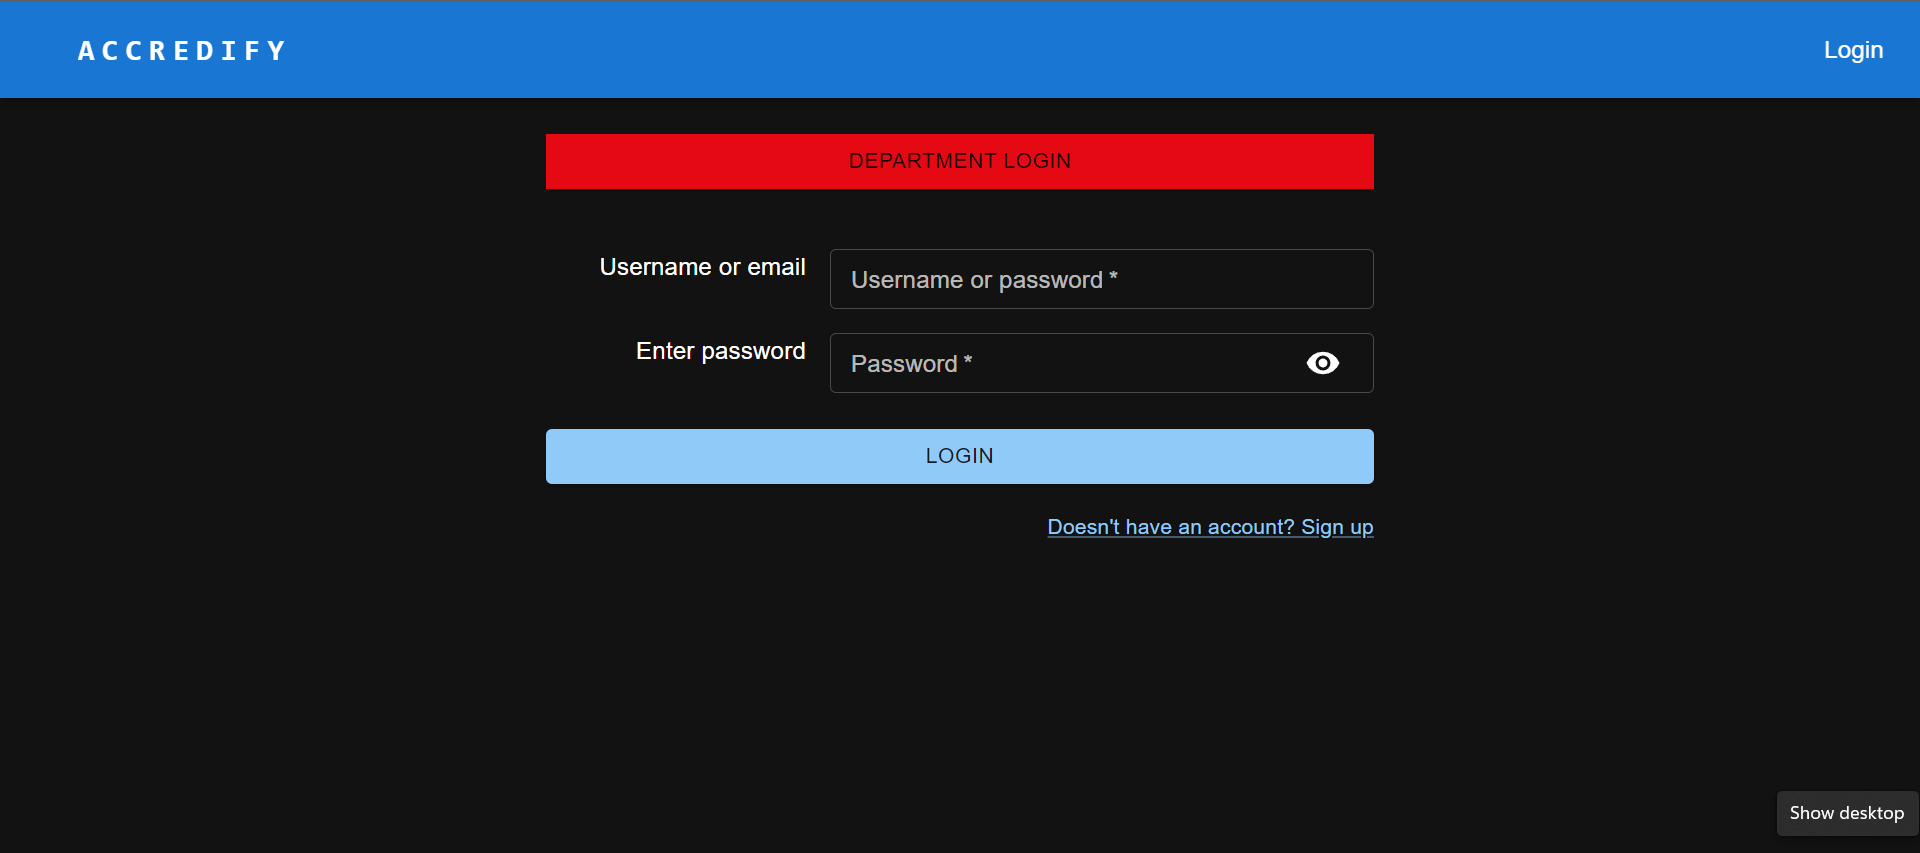
\includegraphics[width=.70\linewidth]{accredify1.png}
	\label{fig:logo.png}
\end{figure}

\section{Sign Up}
If the department doesn't have an account, they need to register. Departments can register using college name, department name, username, email and password. The already registered departments, username and email cannot be duplicated. After signup you will be direced to the pre qualification checking page. 
\begin{figure}[h]
	\centering
	\hspace{21pt}
	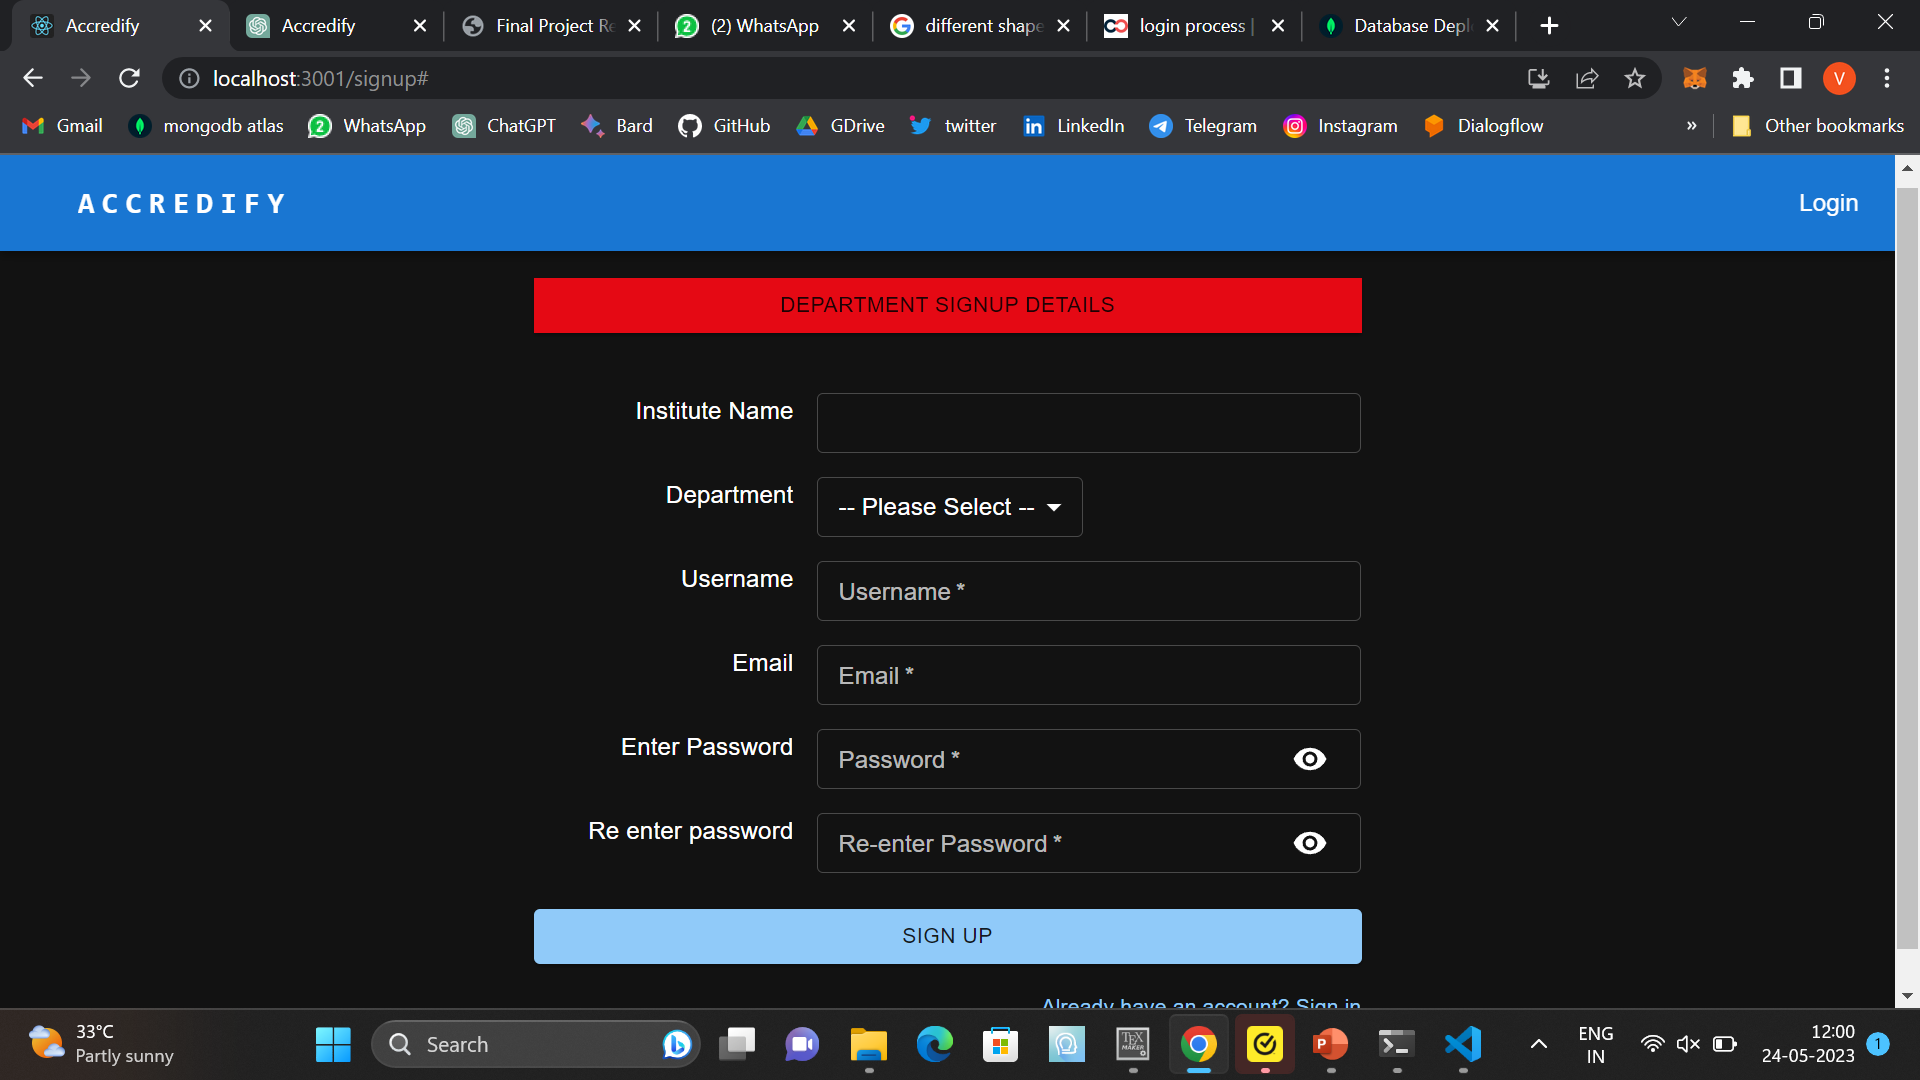
\includegraphics[width=.70\linewidth]{accredify2.png}
	\label{fig:logo.png}
\end{figure}

\section{Pre Qualifiers}
There are certain conditions for the qualification of a department such as student faculty ratio, faculty PhD ratio, student graduation rate etc. You can check it here. 
\begin{figure}[h]
	\centering
	\hspace{21pt}
	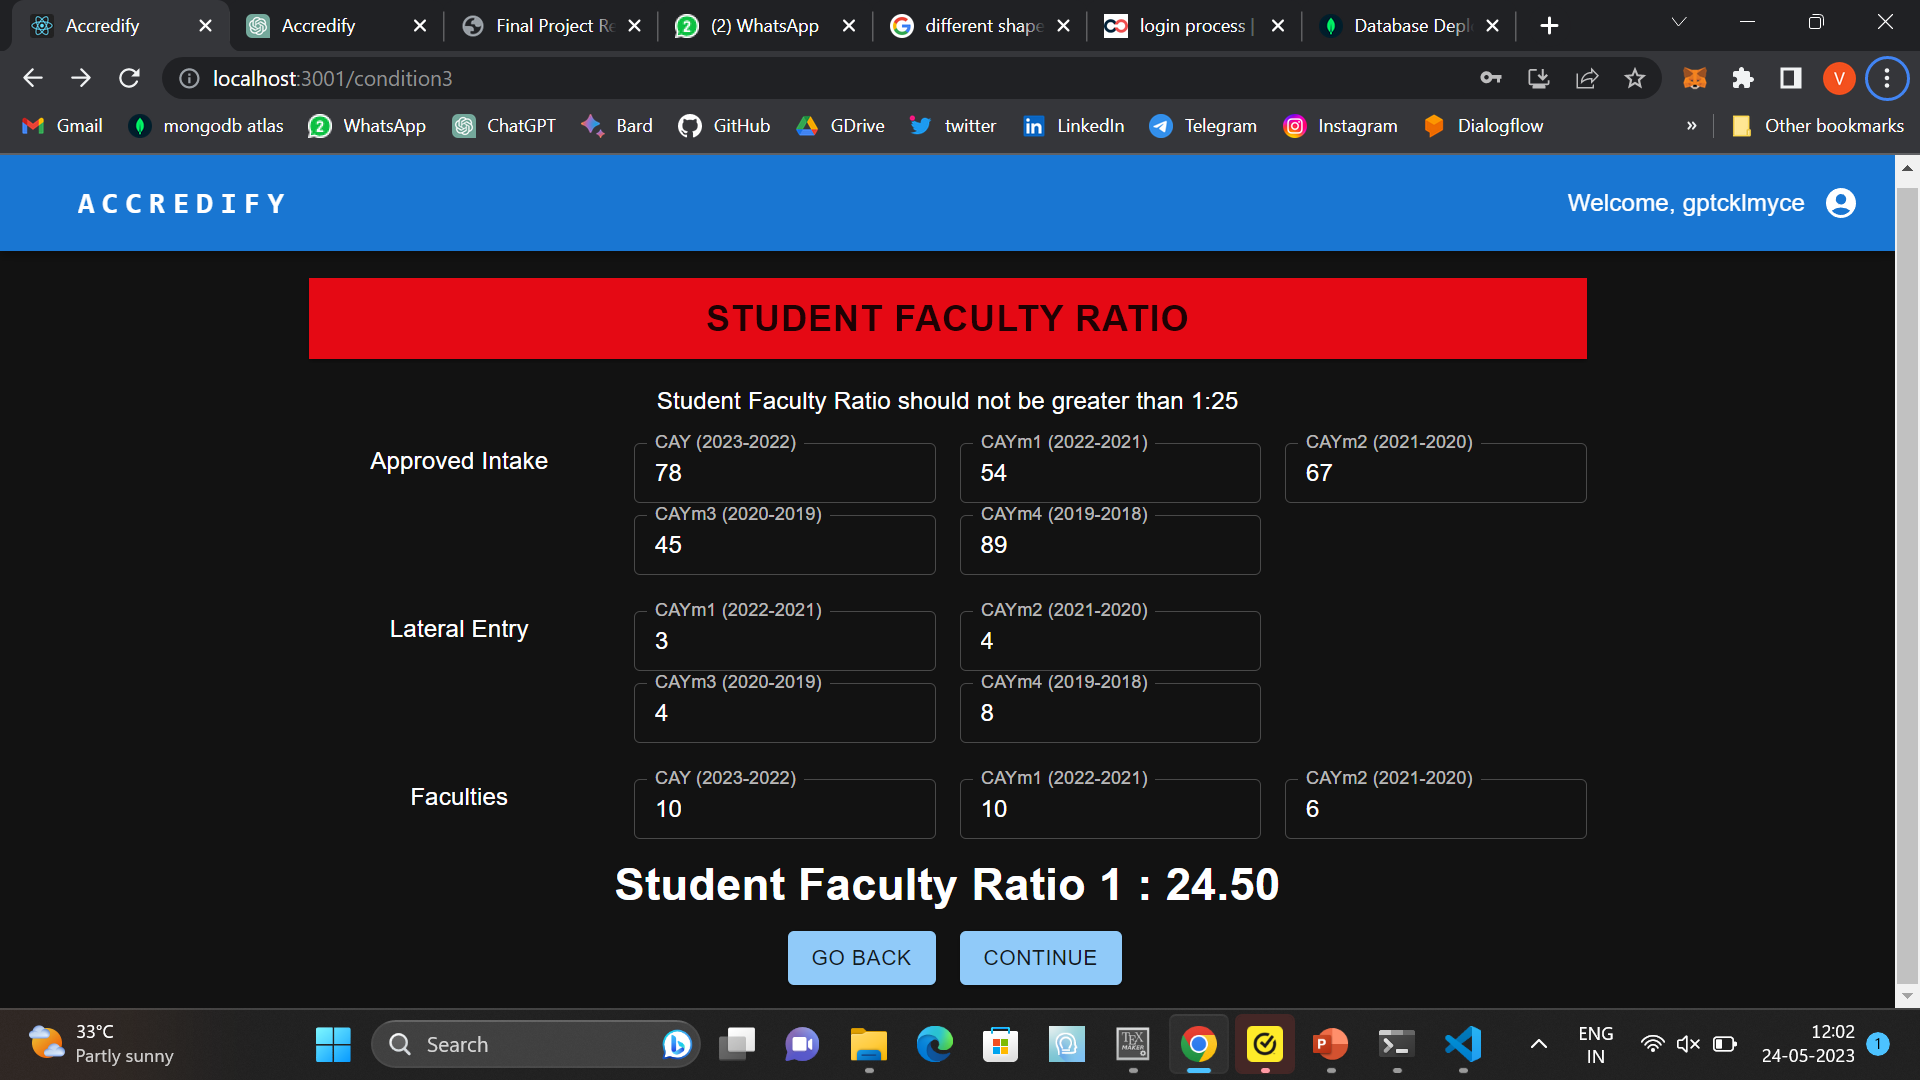
\includegraphics[width=.70\linewidth]{accredify3.png}
	\label{fig:logo.png}
\end{figure}

\section{Premium}
Our website also provides premium services. Advanced consultation services will be provided by our company if the department is a premium member. Razorpay is used for the payment i
\begin{figure}[h]
	\centering
	\hspace{21pt}
	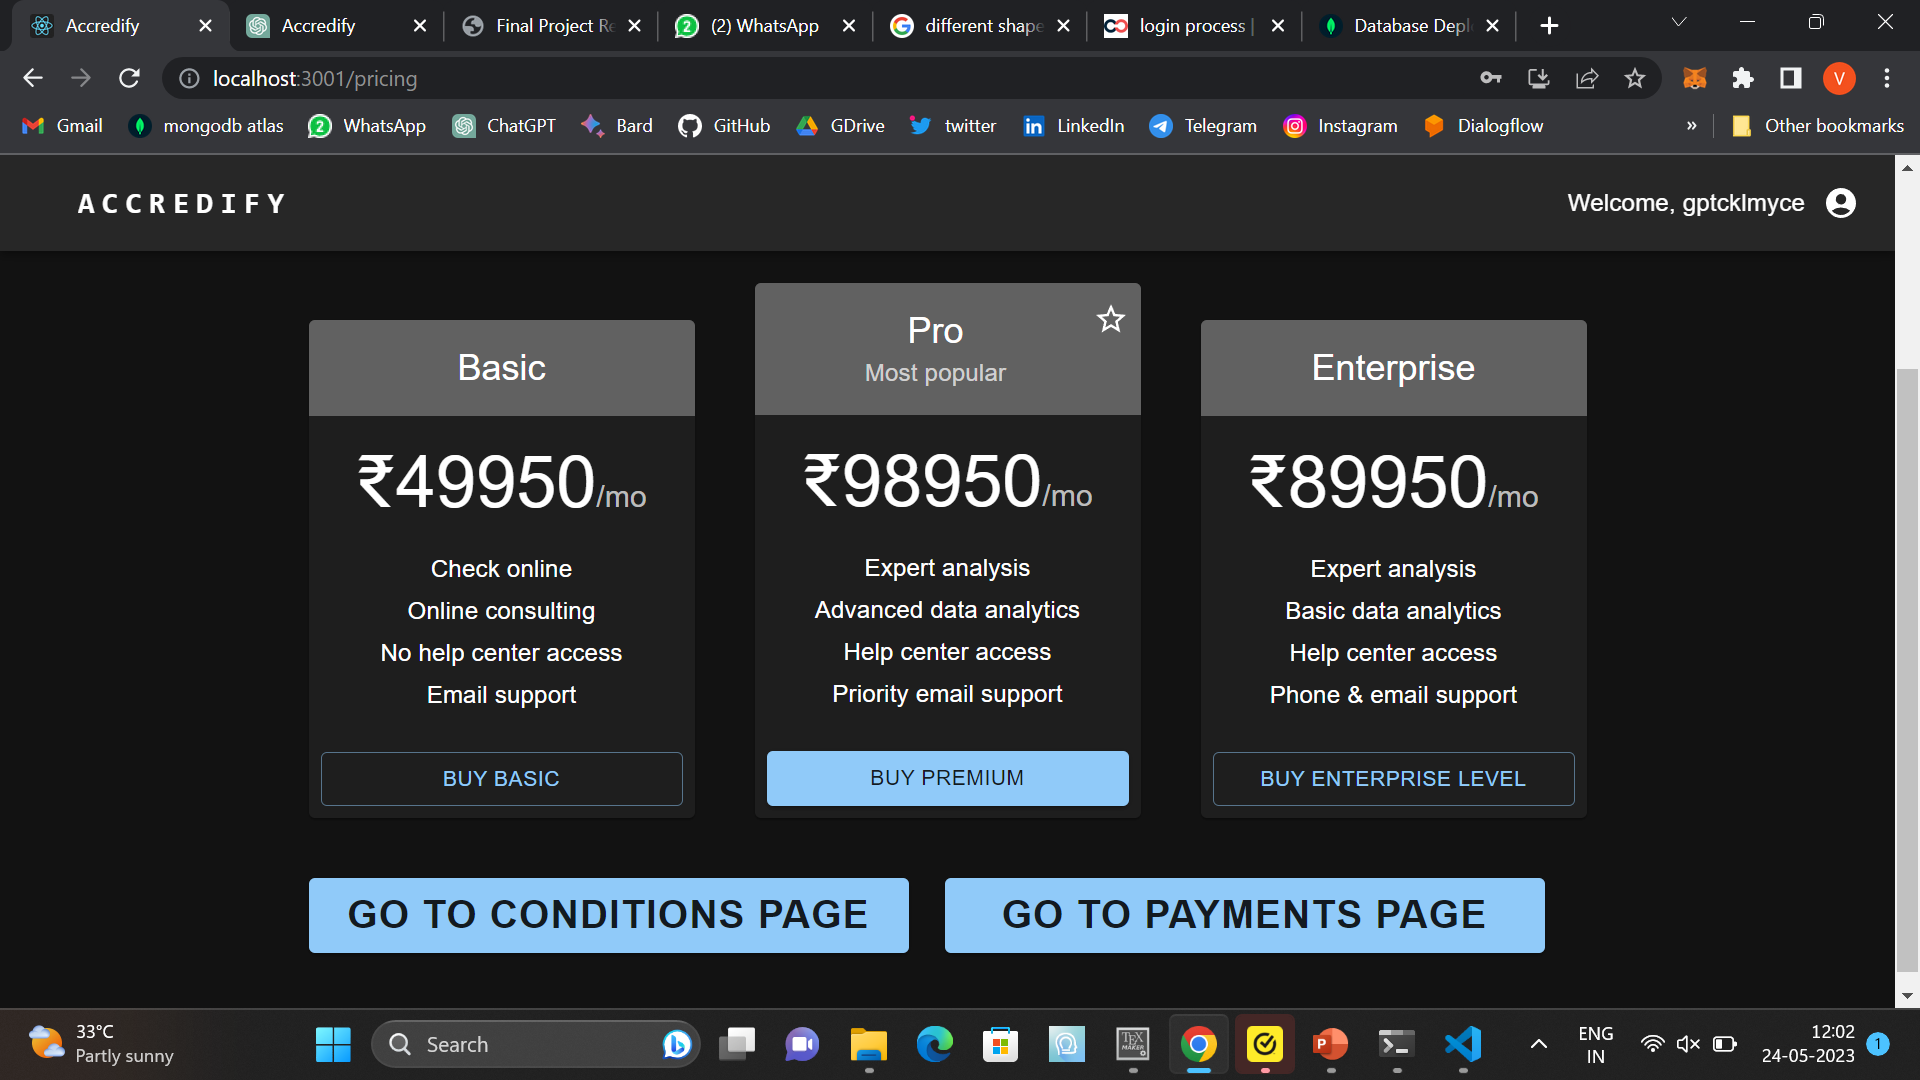
\includegraphics[width=.70\linewidth]{accredify4.png}
	\label{fig:logo.png}
\end{figure}
\section{Razorpay}
Razorpay is used to implement payment.
\begin{figure}[h]
	\centering
	\hspace{21pt}
	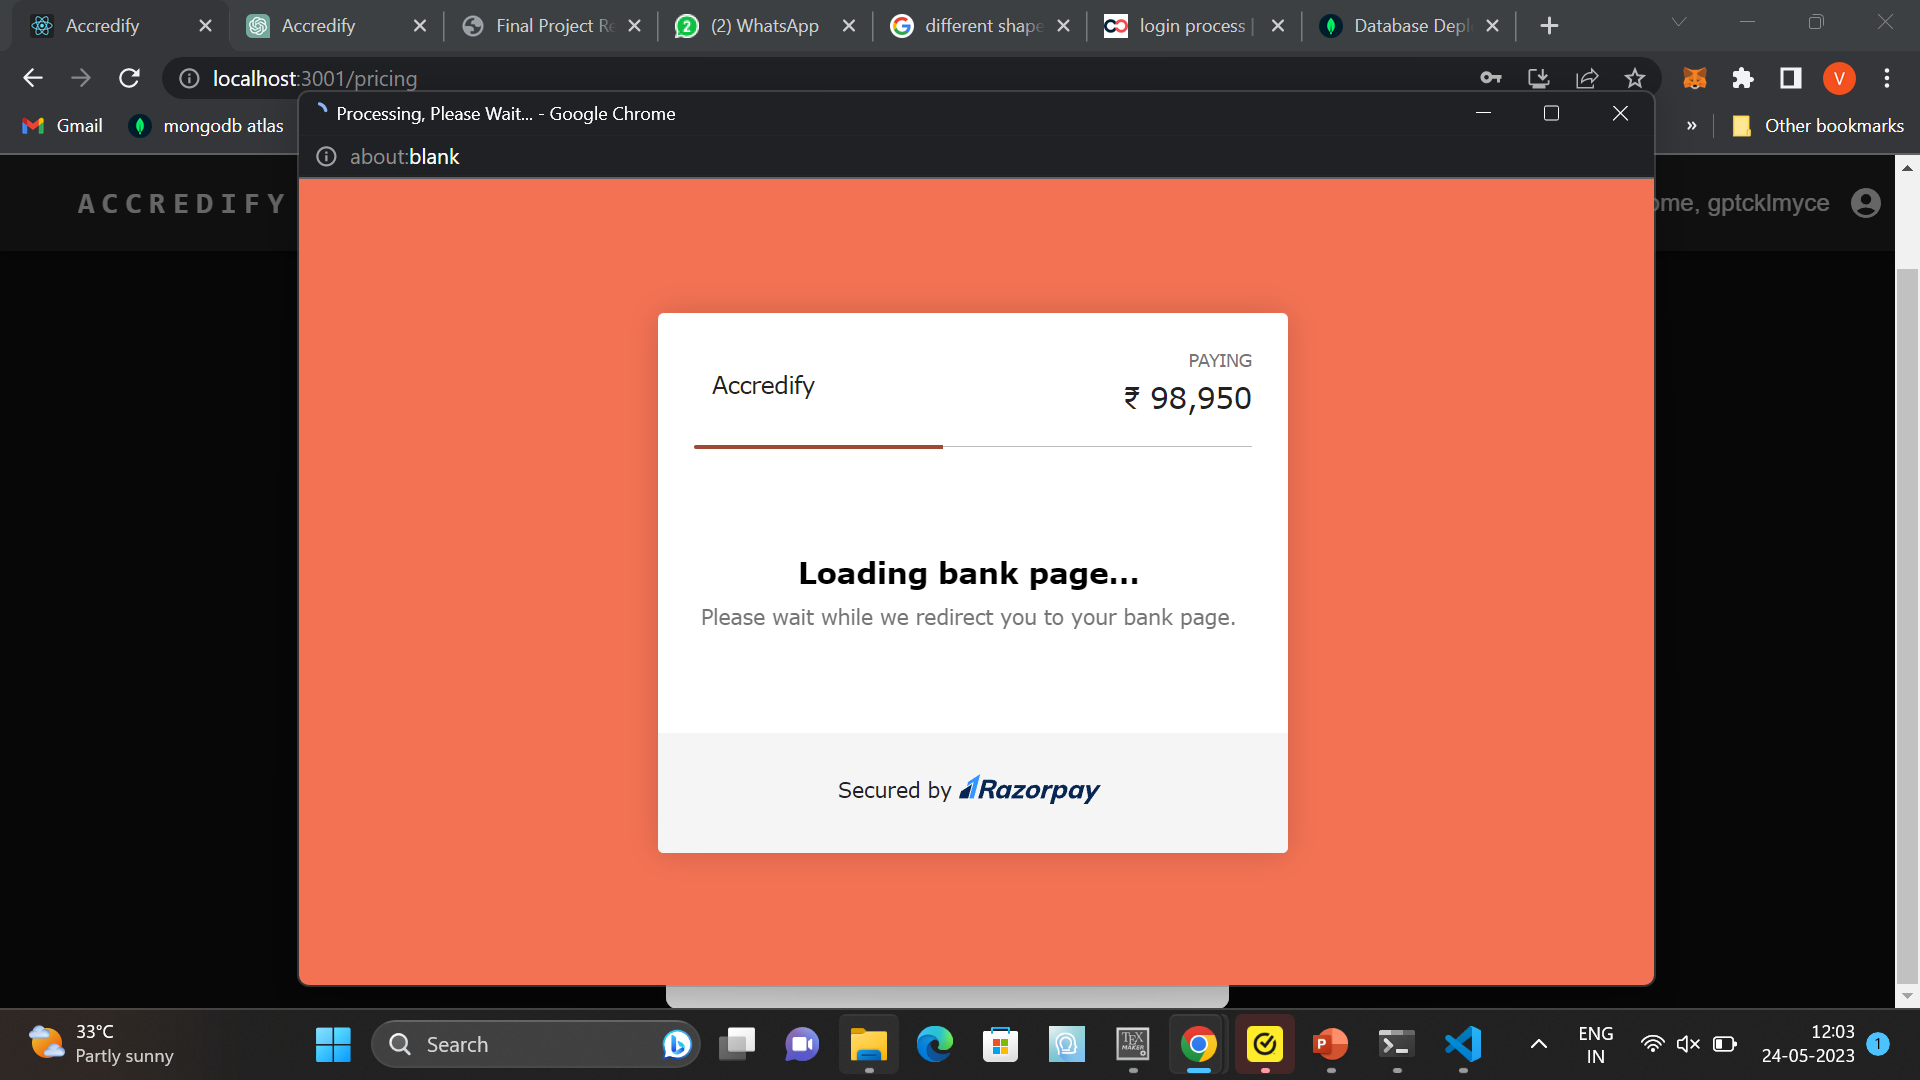
\includegraphics[width=.70\linewidth]{accredify6.png}
	\label{fig:logo.png}
\end{figure}

\section{Invoice Bill}
Departments can print the transaction bill after each payments.
\begin{figure}[h]
	\centering
	\hspace{21pt}
	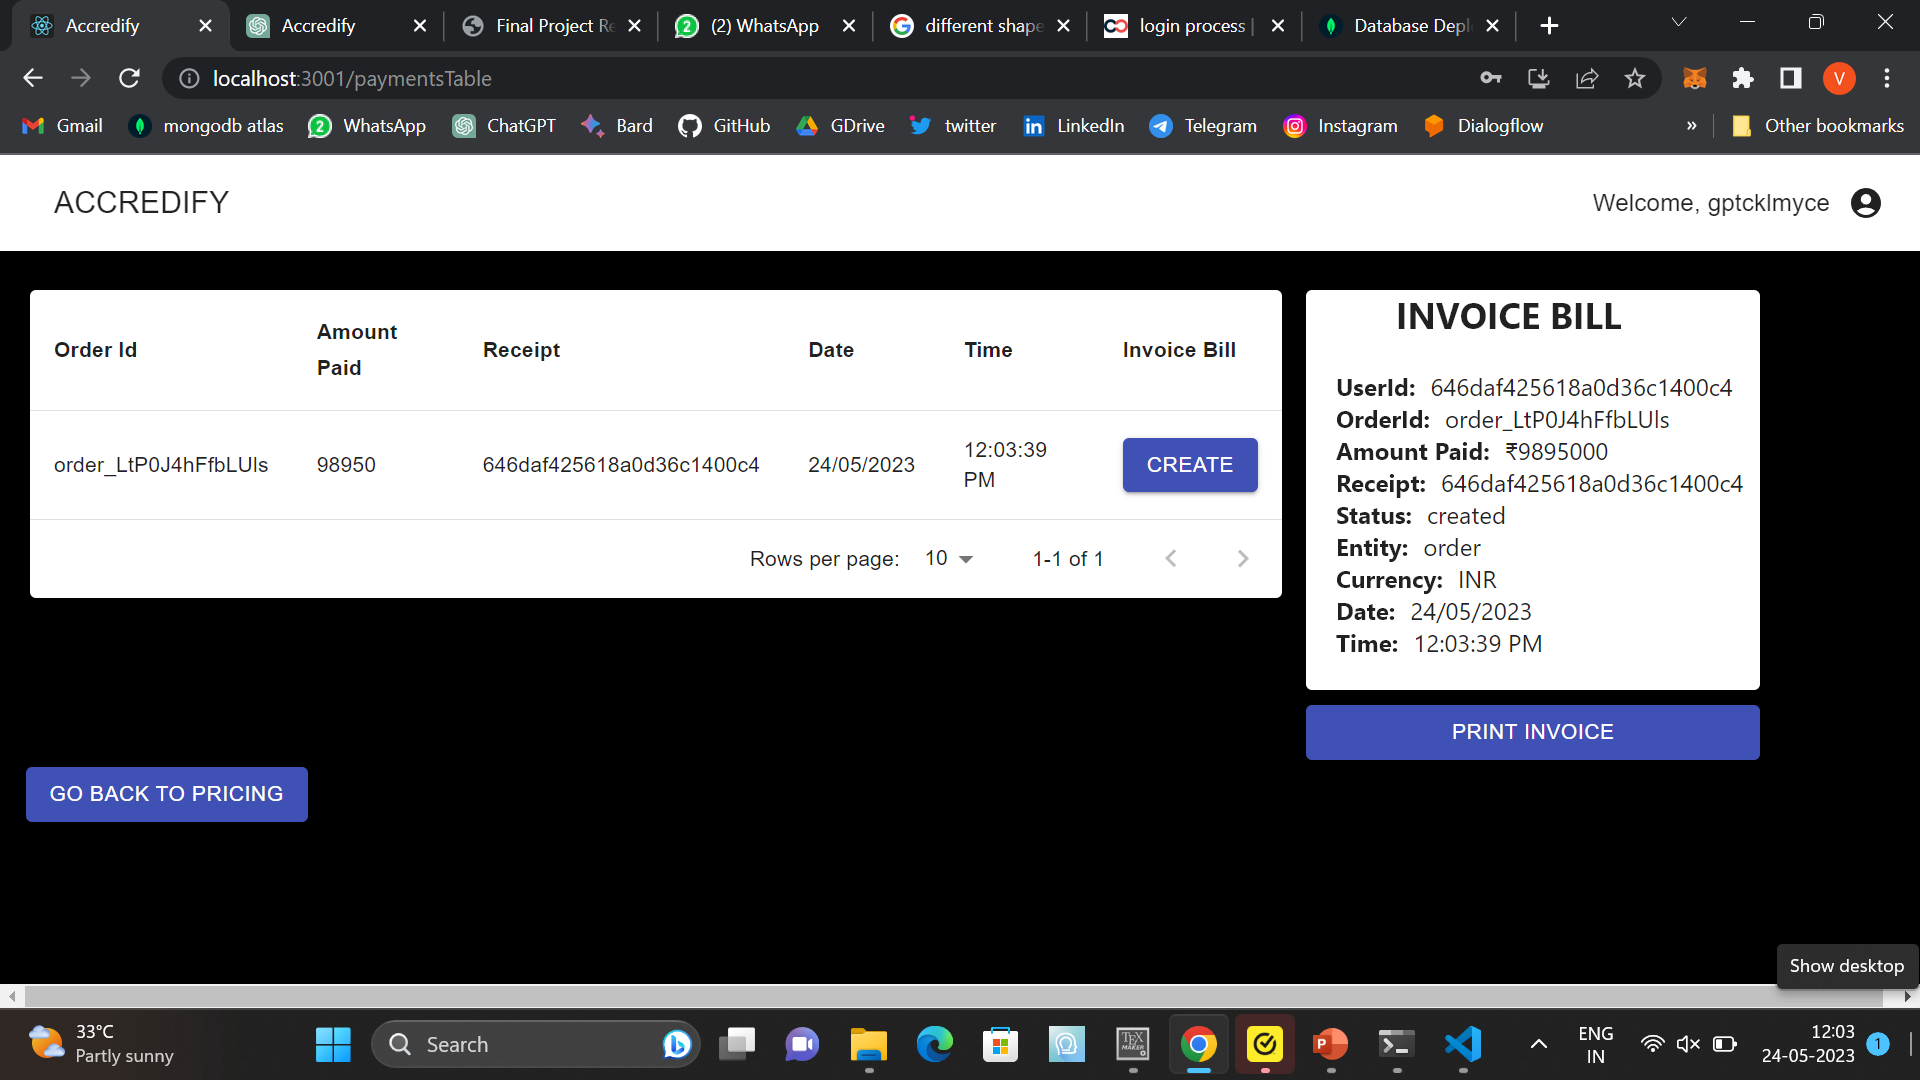
\includegraphics[width=.70\linewidth]{accredify8.png}
	\label{fig:logo.png}
\end{figure}
\begin{figure}[h]
	\centering
	\hspace{21pt}
	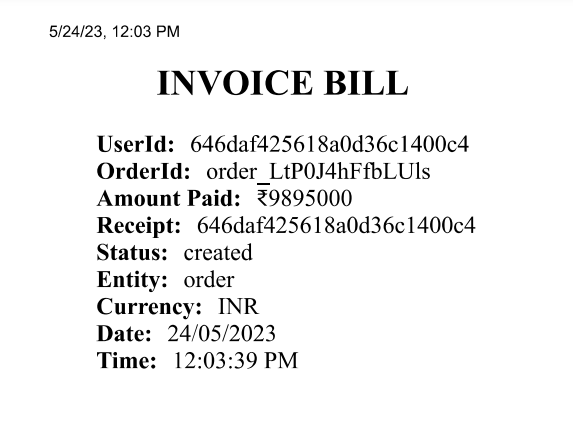
\includegraphics[width=.70\linewidth]{accredify10.png}
	\label{fig:logo.png}
\end{figure}

\section{Admin Dashboard}
This is exclusive for admins. Admins can visualize the data of the departments. Pie charts, bar charts and graph charts are available. The revenue of the company, details of the departments registered is visible in the admin dashboard. 
\begin{figure}[h]
	\centering
	\hspace{21pt}
	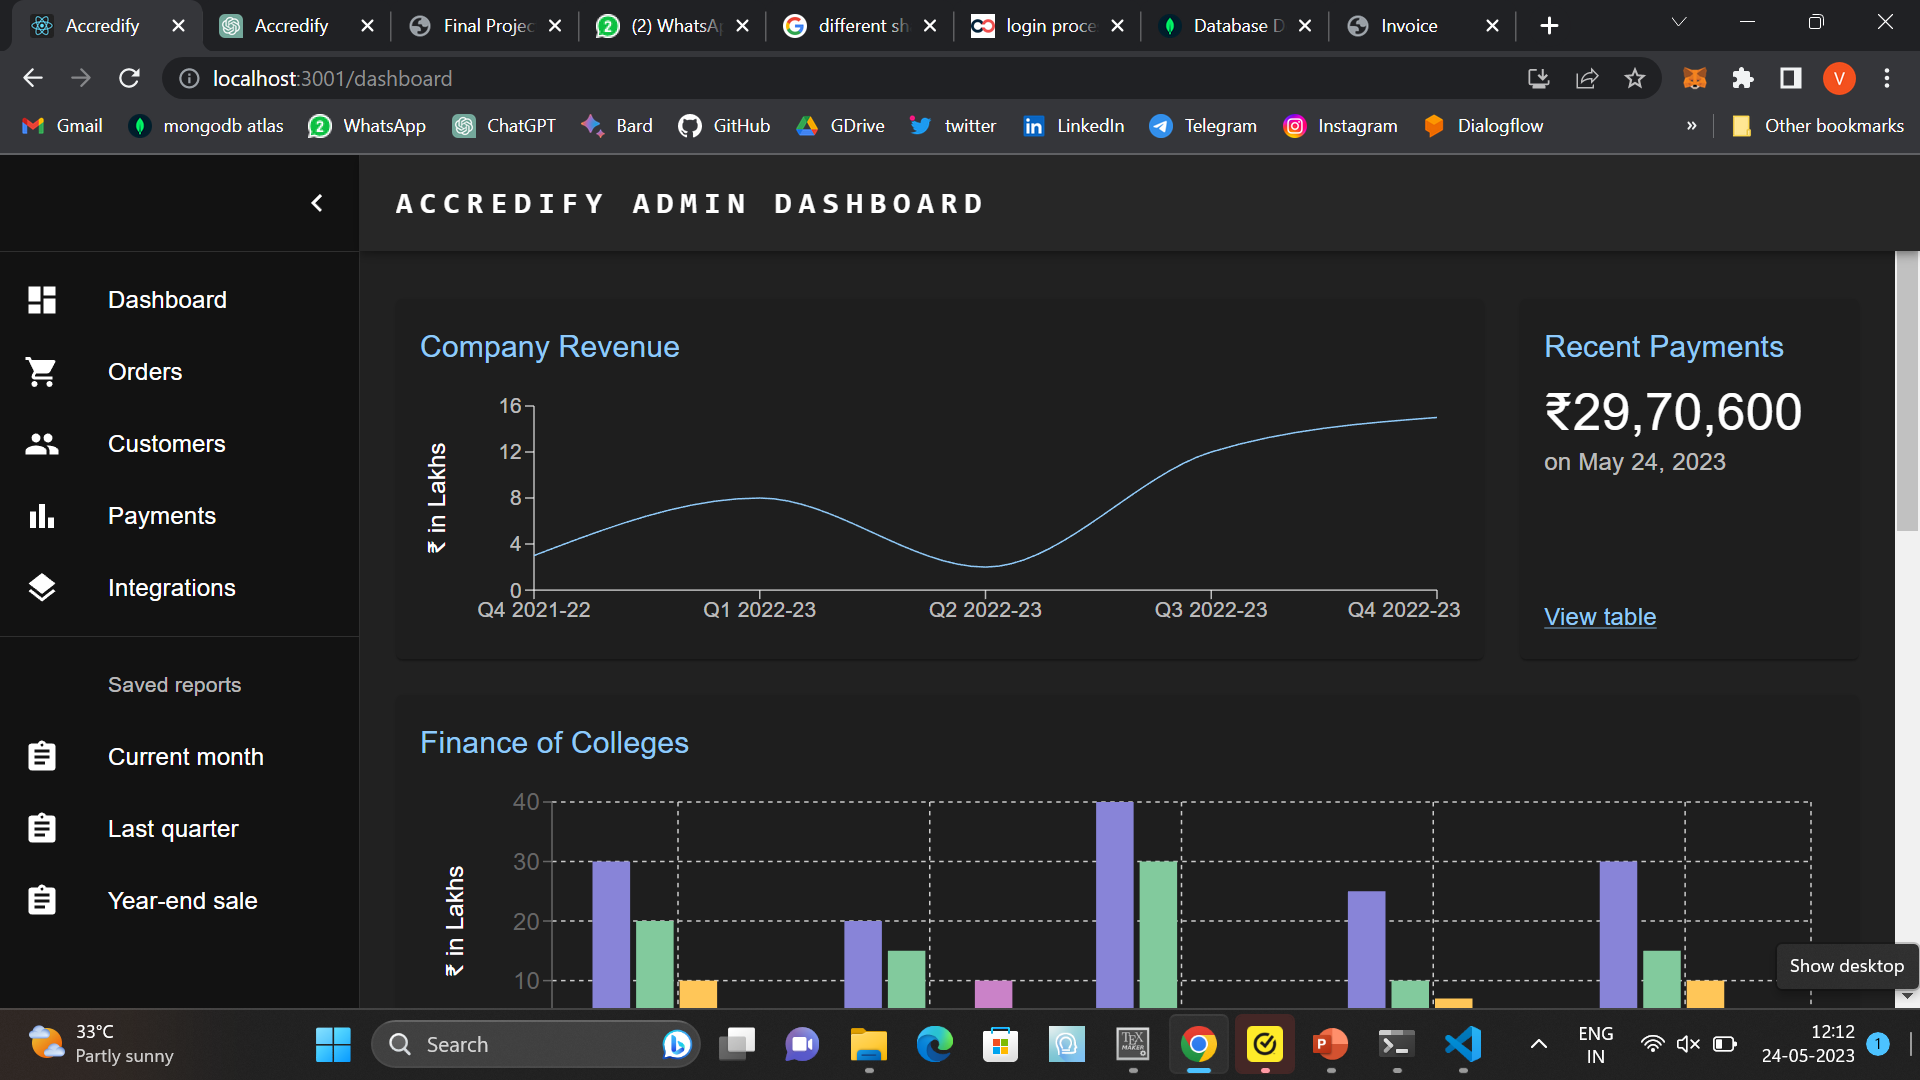
\includegraphics[width=.70\linewidth]{accredify11.png}
	\label{fig:logo.png}
\end{figure}
\begin{figure}[h]
	\centering
	\hspace{21pt}
	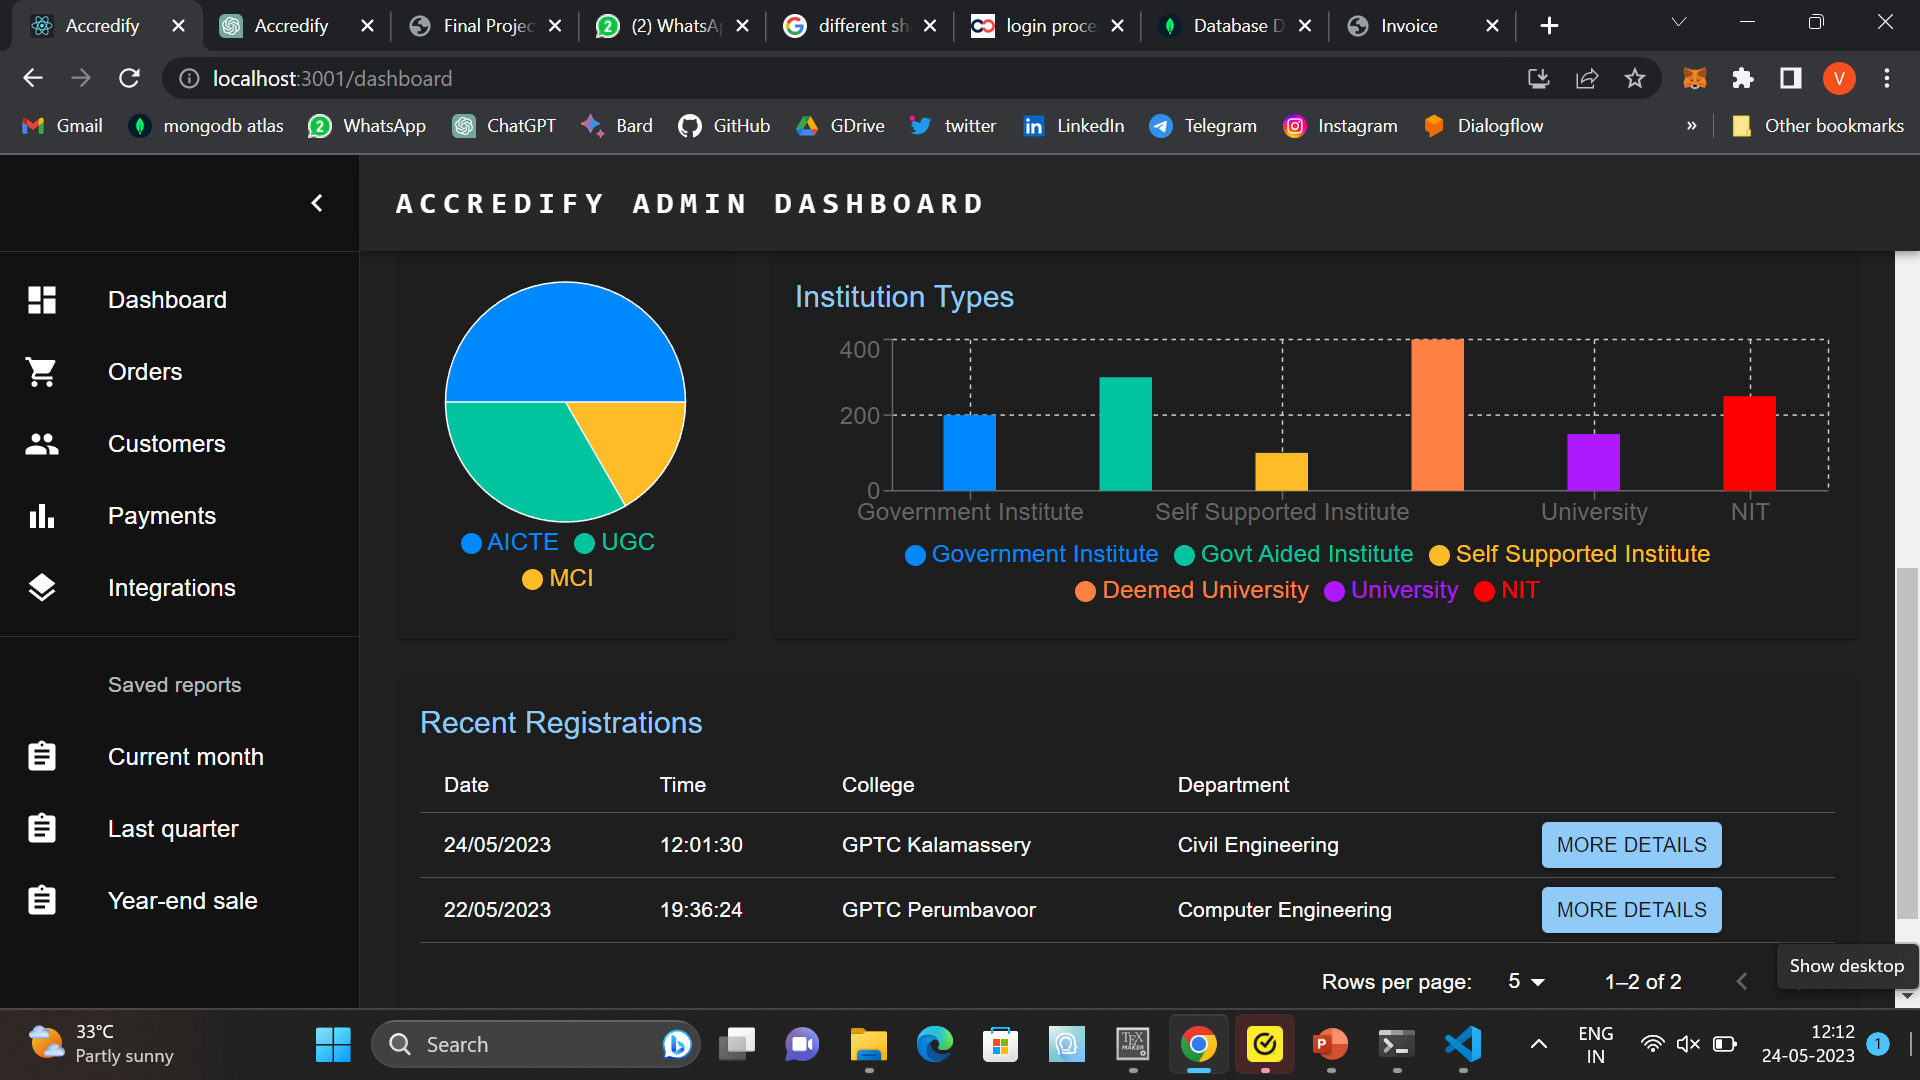
\includegraphics[width=.70\linewidth]{accredify12.png}
	\label{fig:logo.png}
\end{figure}
\begin{figure}[h]
	\centering
	\hspace{21pt}
	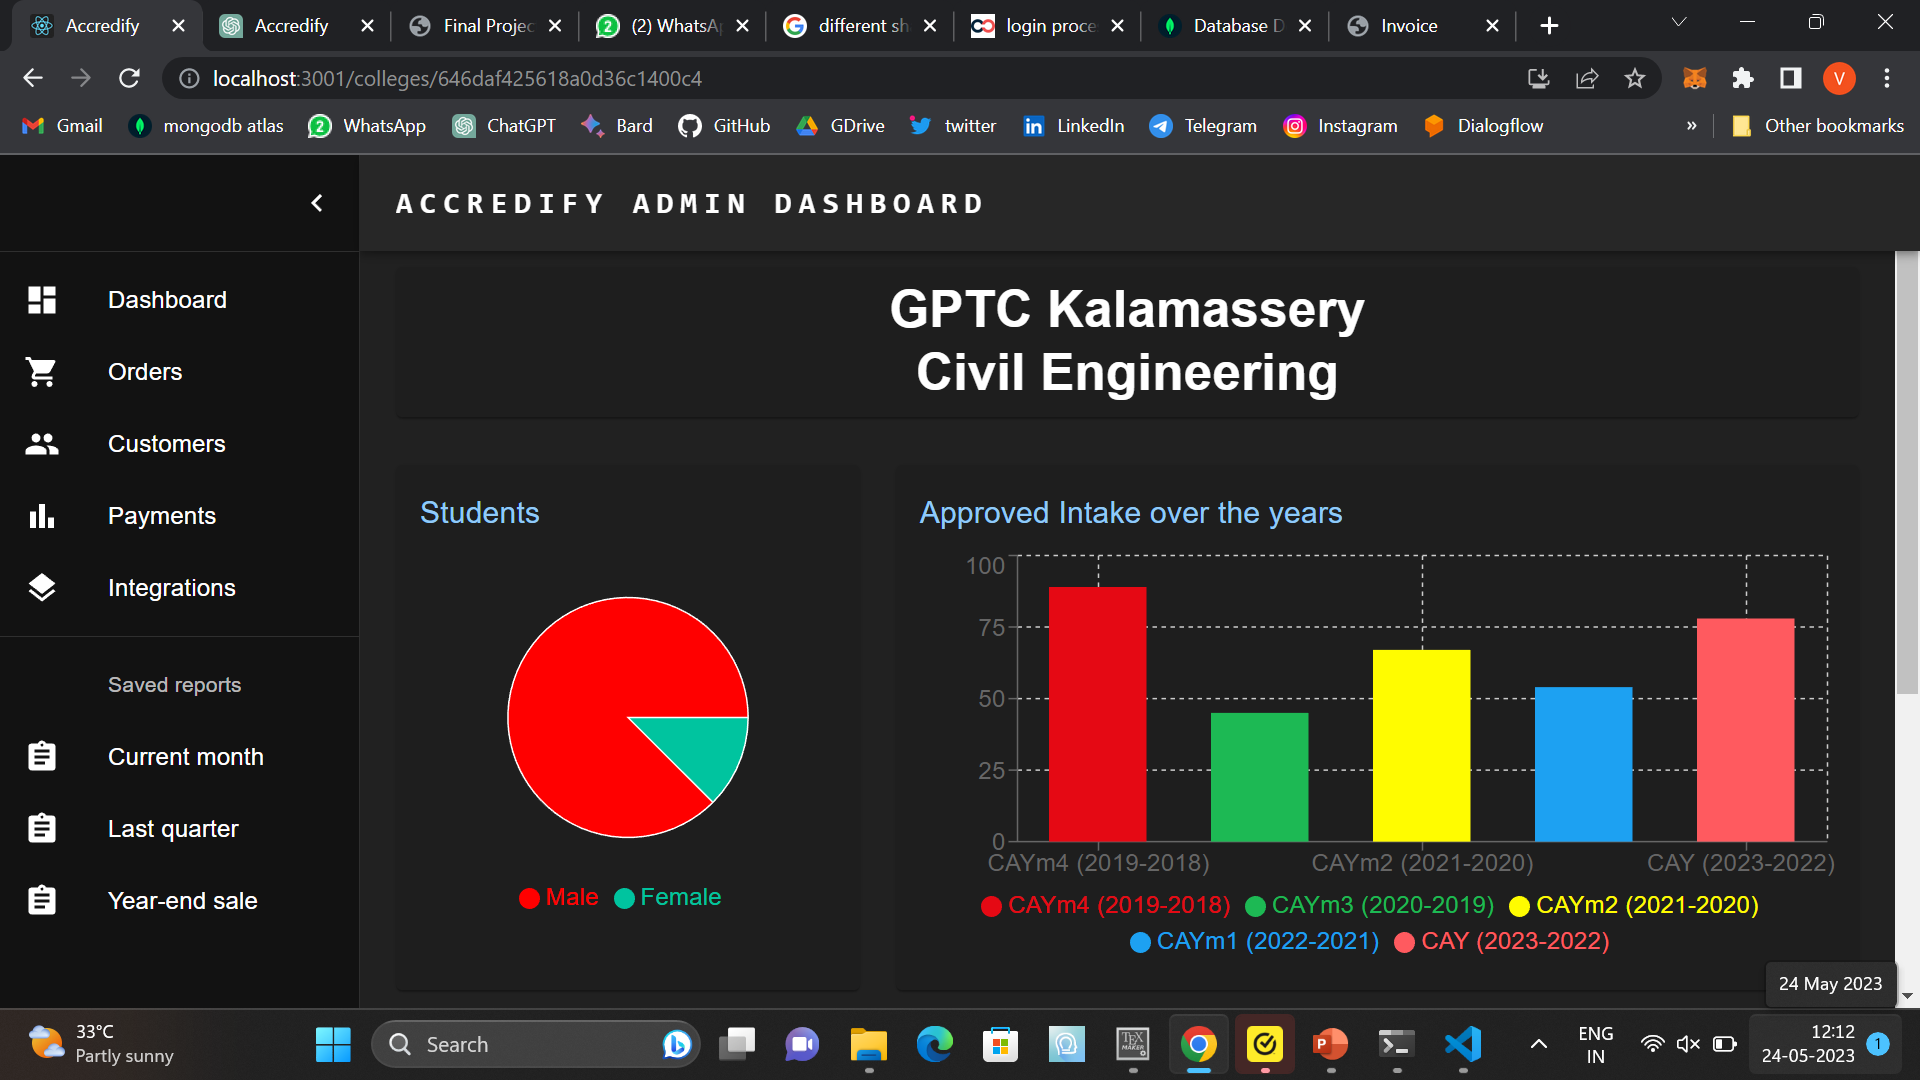
\includegraphics[width=.70\linewidth]{accredify13.png}
	\label{fig:logo.png}
\end{figure}
\begin{figure}[h]
	\centering
	\hspace{21pt}
	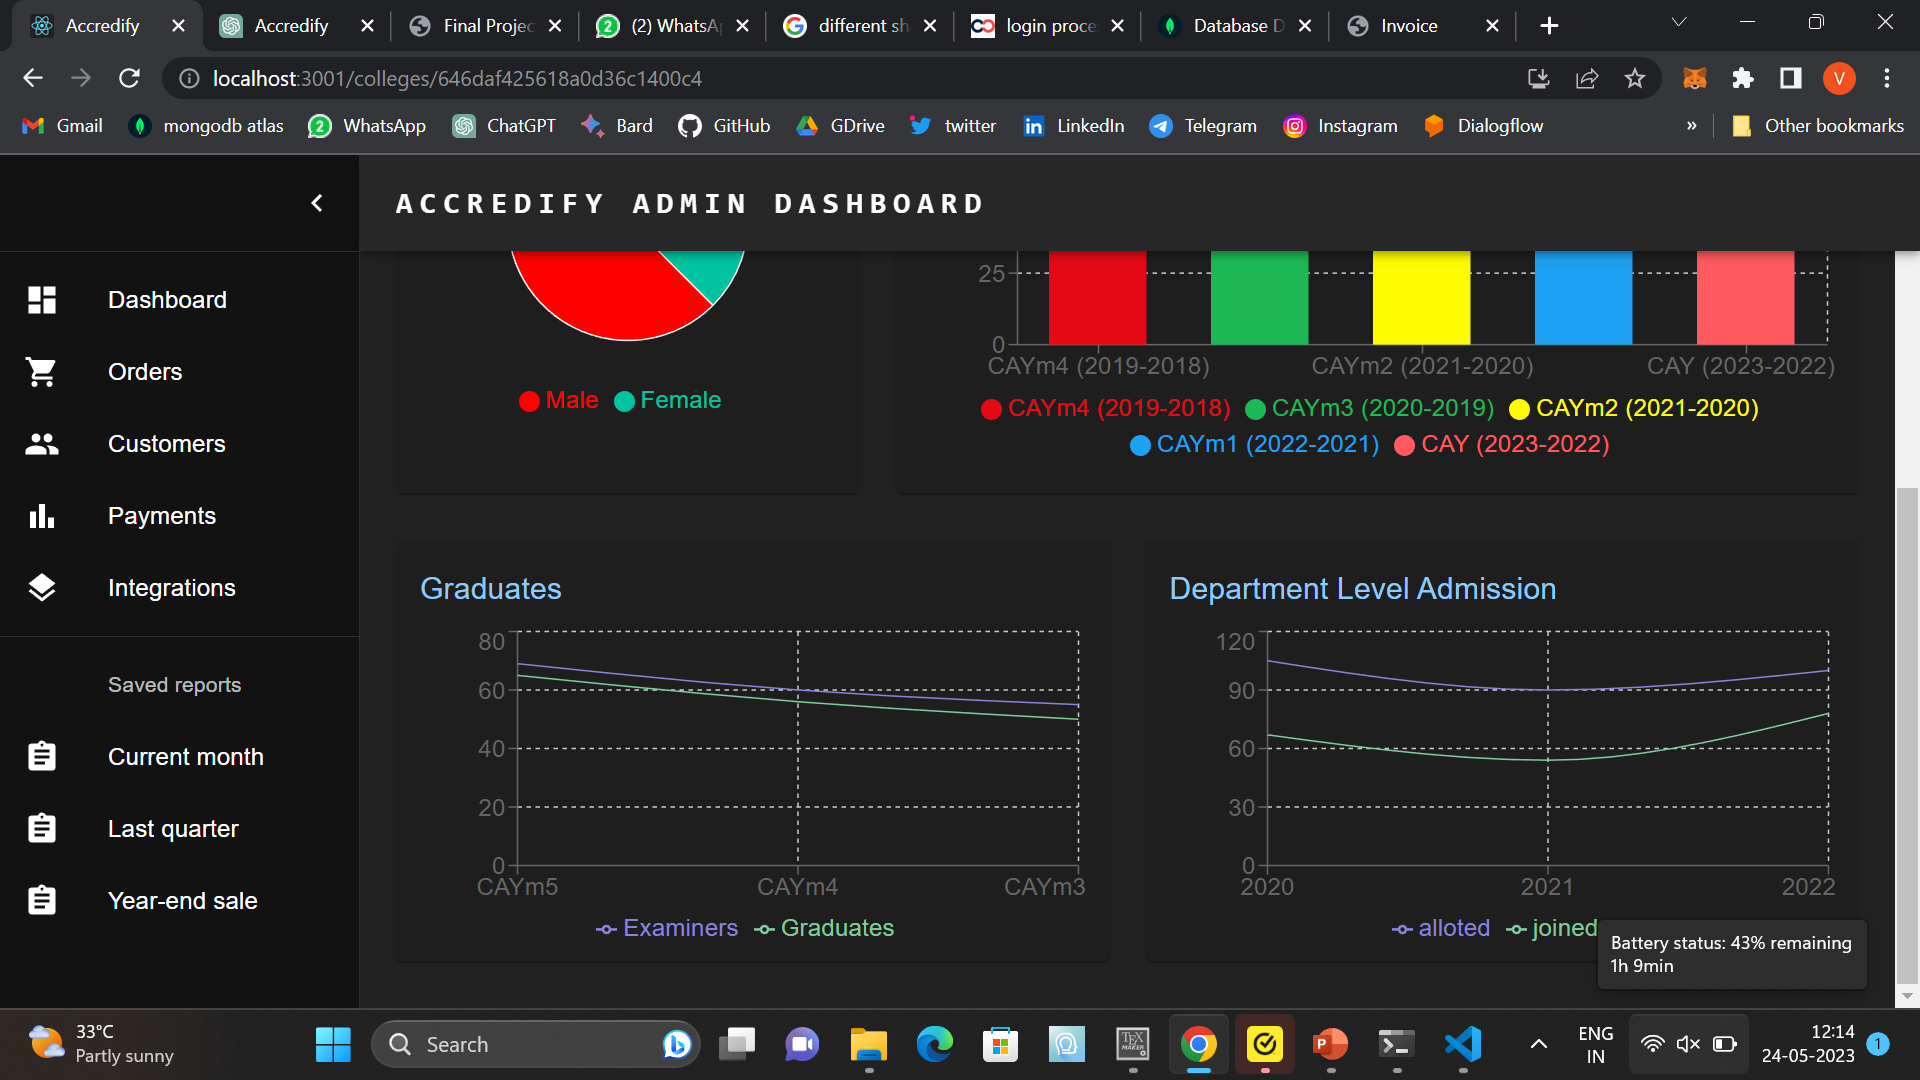
\includegraphics[width=.70\linewidth]{accredify14.png}
	\label{fig:logo.png}
\end{figure}




\chapter{Conclusion}
In conclusion, the development of this application has been driven by a set of clear objectives that have guided the entire process. By addressing a specific problem or need, the application aims to provide a valuable solution that meets the requirements and preferences of its users. The focus on enhancing user experience has resulted in intuitive interfaces, smooth navigation, and visually appealing elements that create a seamless and enjoyable interaction for users.

Reliability and performance have been prioritized, ensuring that the application operates efficiently and minimizes downtime or errors. The implementation of robust security measures underscores the commitment to protecting user data and maintaining their privacy. Scalability and maintainability have also been considered, allowing the application to adapt and grow alongside changing user demands and technological advancements.

By aligning with business goals, the application contributes to the organization's success, whether through revenue generation, customer expansion, or operational improvements. Through these objectives, the development of the application has been driven by a clear vision and purpose, ensuring that it delivers value to its users and remains relevant in the long run.

Overall, the successful achievement of these objectives demonstrates the dedication and commitment of the development team, stakeholders, and all involved in the creation of the application. With the objectives as the guiding force, the application is poised to make a positive impact, provide value, and meet the needs of its users, contributing to their success and satisfaction.

\chapter{References}

\begin{itemize}
\item Pro MERN Stack \\
  \url{https://link.springer.com/book/10.1007/978-1-4842-4391-6}
  

  \item MERN Stack Web Development \\
  \url{https://www.annalsofrscb.ro/index.php/journal/article/view/7719}

  \item Accreditation system for technical education programmes in India: A critical review \\
  \url{https://www.tandfonline.com/doi/abs/10.1080/03043790903497294}
  
  \item Seaborn: Statistical data visualization \\
  \url{https://joss.theoj.org/papers/10.21105/joss.03021.pdf}
\vspace{12pt}

\item Effectiveness of NBA accreditation processes \\
  \url{https://citeseerx.ist.psu.edu/document?repid=rep1&type=pdf&doi=e7223fd9946ca8a76bc188f84fa71753f7836b57#page=100}
\vspace{12pt}
\end{itemize}
\end{document}
